\chapter{Results}
\label{sec:results}

\begin{figure*}[h!t]
	\centering
	
	\subfloat[LuxRender]{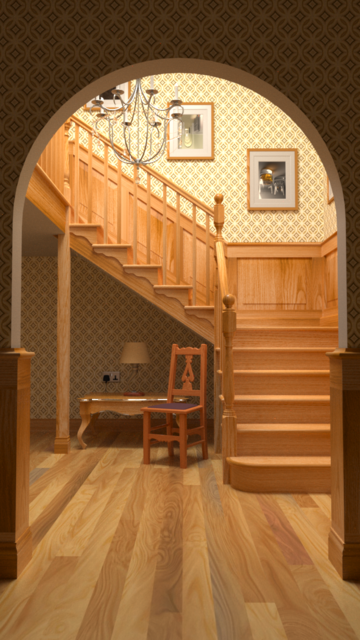
\includegraphics[width=0.32\linewidth]{images/5_results/staircase/1_from_lux.png}
		\label{staircase_Lux}
	}
	\subfloat[PBRT v3]{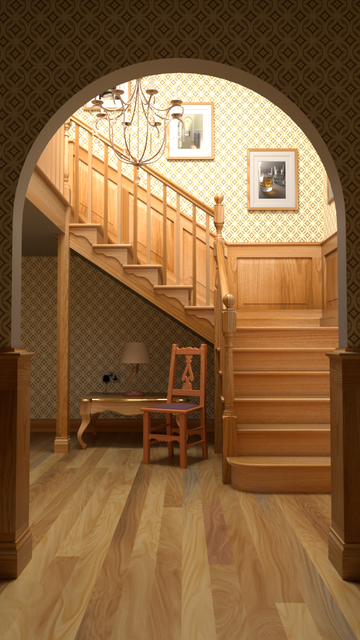
\includegraphics[width=0.32\linewidth]{images/5_results/staircase/3_to_pbrt.png}
		\label{staircase_PBRT}
	}
	\subfloat[Mitsuba]{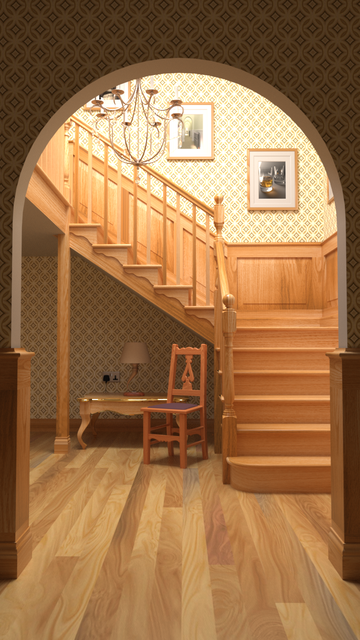
\includegraphics[width=0.32\linewidth]{images/5_results/staircase/2_to_mitsuba.png}
		\label{staircase_Mitsuba}
	}
	\caption{\textit{The Wooden Staircase} scene. Input scene description for LuxRender (a).
		Renderings produced by PBRT v3 (b) and Mitsuba (c),
		from scene descriptions converted by our system. }
	\label{fig:staircase}
\end{figure*}

Our system is available on-line~\cite{sceneConverter}.
We have tested it on a large number of scenes, including the 32 scenes available
at Bitterli's rendering resources website~\cite{resources16}. 
%We validated our system's conversion using scenes from Bitterli's 32 resources 
%\cite{resources16}. 
Here, we include a few examples to illustrate its results on scenes that explore different 
types of materials, 3D meshes and primitive shapes, image and 
procedural textures, and various lighting styles. They include most elements typically found in scenes used by physically-based rendering systems.  The time required to convert a scene is about 0.5 seconds on a typical PC (Intel i5 3.8 GHz).
% 
%We chose scenes that provided a wide variety of directives 
%in order to cover most commonly used directives. These scenes include: different 
%types of materials and bump maps; 3D meshes and primitive shapes; image and 
%primitive textures; area and environment lighting. 
%
The scenes were rendered using Mitsuba 0.5.0, PBRT v3, and LuxRender v1.6 on 
Ubuntu 14.04 LTS. All scenes were rendered using between 5,000 and 8,000 samples per pixel (spp). For any given scene,
the same number of samples per pixel was used with all rendering systems. 

Figure~\ref{fig:teaser} shows a coffee maker containing various materials, including glass, plastic, and metal, as well as textures. The input scene description was provided in the format for PBRT v3, whose rendering is shown on the left. The images at the center and on the right were produced by Mitusuba and LuxRender, respectively, from scene representations automatically converted by our system. 
%from the input scene file. 
Note how the object details have been faithfully preserved in these renderings.

The \textit{Wooden Staircase} scene (Figure~\ref{fig:staircase}) contains many geometric objects and textures. 
A LuxRender scene description was provided as input and its rendering is shown in (a). The images shown in (b) and (c) were produced 
by PBRT v3 and Mitsuba, respectively, from scene representations automatically converted by our system. 

The \textit{Teapot} scene (Figure \ref{fig:teapot}) contains a shiny object, environment lighting, and a procedural texture. The input scene description was also provided in the LuxRender format. Figures~\ref{teatpot_PBRT} and \ref{teapot_Mitsuba} show the renderings produced by PBRT v3 and Mitsuba, respectively, from scene descriptions converted by our system.

Figure~\ref{fig:bidir-cornell} shows two scenes, \textit{Veach Bidir Room} and \textit{Cornell Box}. The first includes caustics, while the second only contains diffuse surfaces. A Mitsuba scene description was provided as input for each of these scenes, whose renderings are shown on the first column of Figure~\ref{fig:bidir-cornell}. Columns (b) and (c) show, respectively, the renderings produced by PBRT v3 and LuxRender using scene descriptions converted by our system.    



\begin{figure*}
\centering

\subfloat[LuxRender]{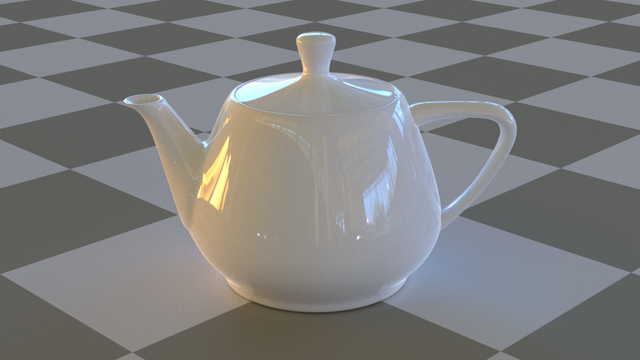
\includegraphics[width=0.32\linewidth]{images/5_results/teapot/1_from_lux.png}
	\label{teapot_Lux}
}
\subfloat[PBRT v3]{\includegraphics[width=0.32\linewidth]{images/5_results/teapot/3_to_pbrt.png}
	\label{teatpot_PBRT}
}
\subfloat[Mitsuba]{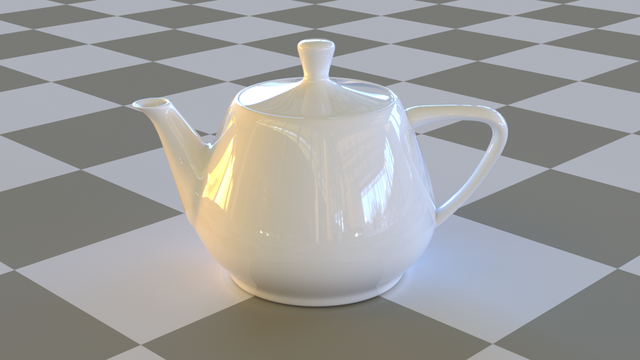
\includegraphics[width=0.32\linewidth]{images/5_results/teapot/2_to_mitsuba.png}
	\label{teapot_Mitsuba}
}
%
%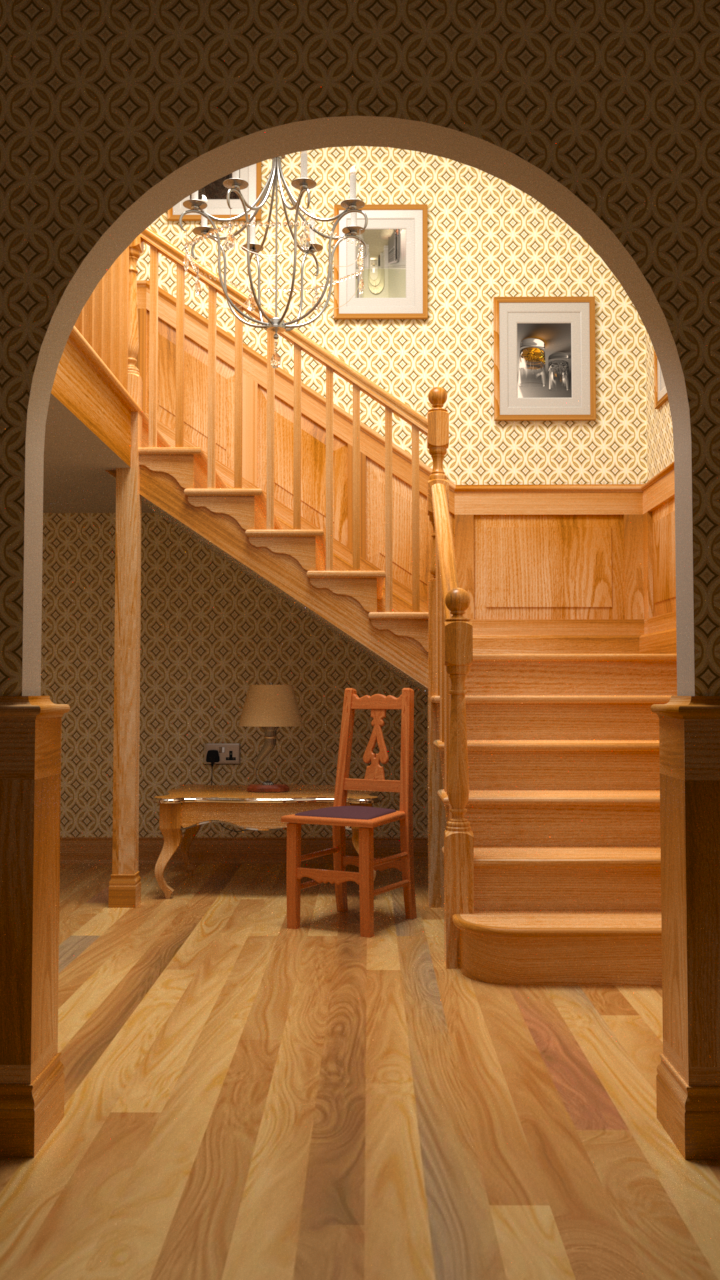
\includegraphics[width=0.32\linewidth]{figs/4_results/teapot/1_from_lux.png}
%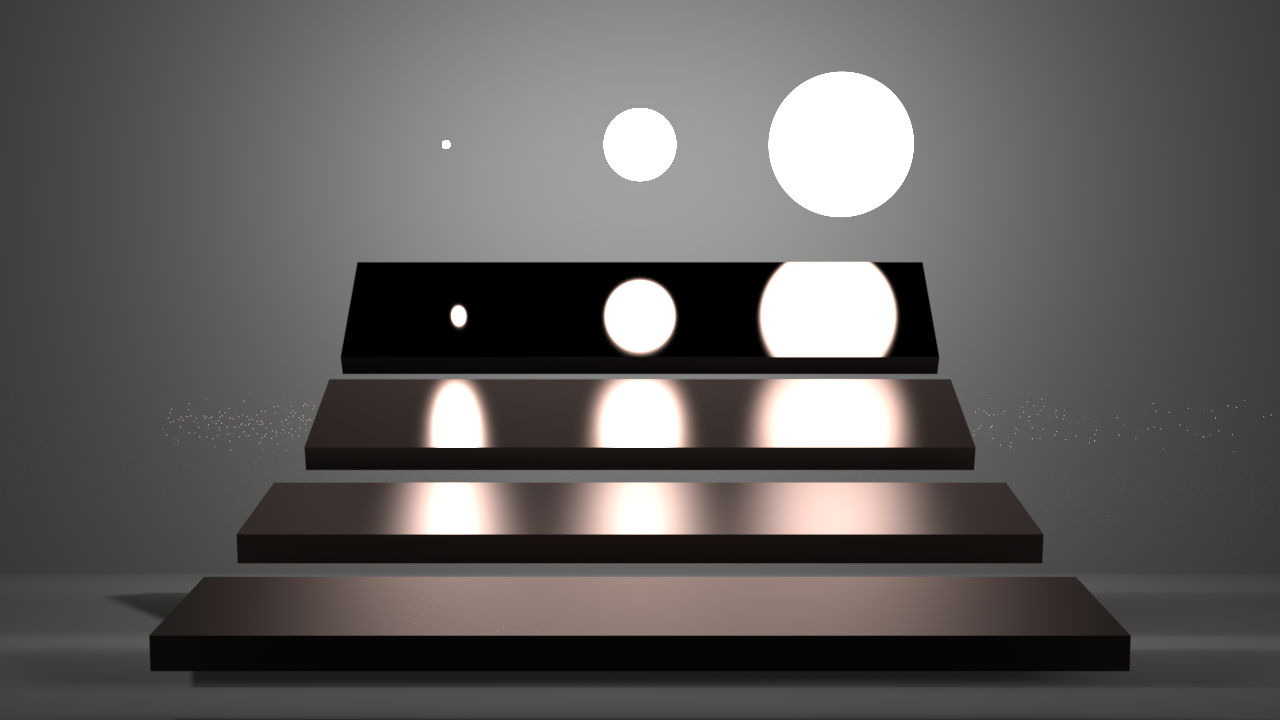
\includegraphics[width=0.32\linewidth]{figs/4_results/teapot/2_to_mitsuba.png}
%\includegraphics[width=0.32\linewidth]{figs/4_results/teapot/3_to_pbrt.png}
\caption{\textit{Teapot} scene. Input scene description for LuxRender (a).	Renderings produced by PBRT v3 (b) and Mitsuba (c),
	from scene descriptions converted by our system.}
\label{fig:teapot}
\end{figure*}

\begin{figure*}
\centering
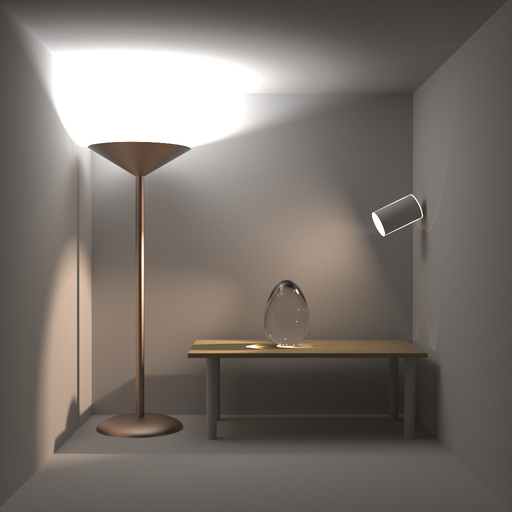
\includegraphics[width=0.32\linewidth]{images/5_results/veach-bidir/1_from_mitsuba.png}
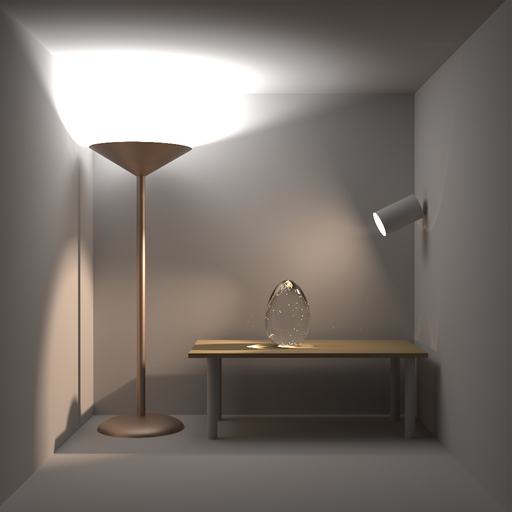
\includegraphics[width=0.32\linewidth]{images/5_results/veach-bidir/2_to_pbrt.png}
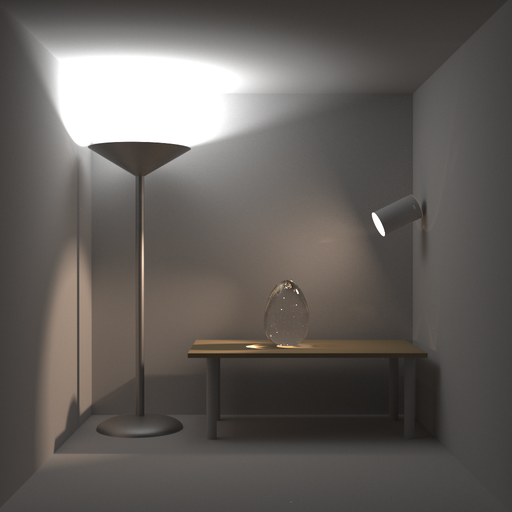
\includegraphics[width=0.32\linewidth]{images/5_results/veach-bidir/3_to_lux.png}
%\vspace{-0.2cm}
\subfloat[Mitsuba]{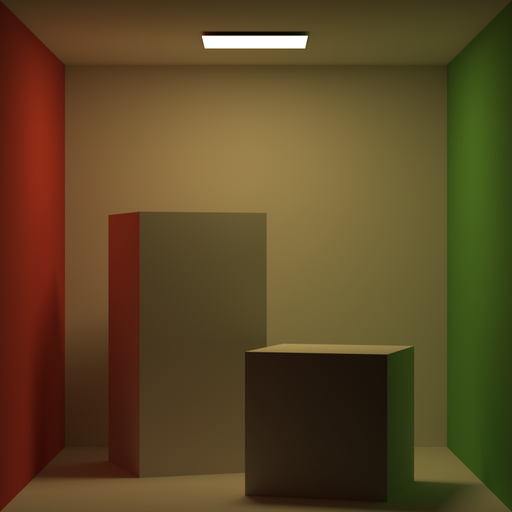
\includegraphics[width=0.32\linewidth]{images/5_results/cornell-box/1_from_mitsuba.png}
}	
\subfloat[PBRT v3]{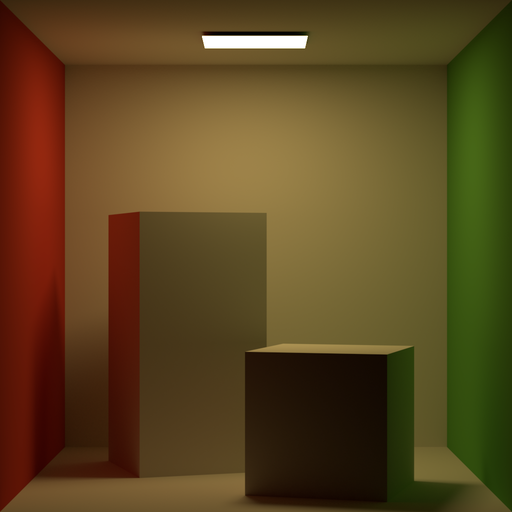
\includegraphics[width=0.32\linewidth]{images/5_results/cornell-box/2_to_pbrt.png}
}	
\subfloat[LuxRender]{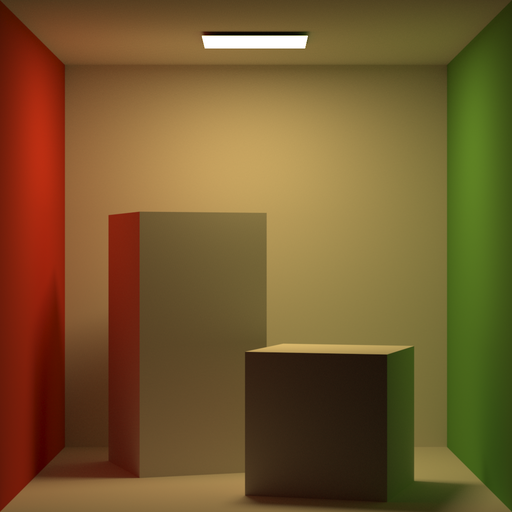
\includegraphics[width=0.32\linewidth]{images/5_results/cornell-box/3_to_lux.png}}
\caption{\textit{Veach, Bidir Room} (top) and \textit{Cornell Box} (bottom). Input scene descriptions for 
 Mitsuba (a). Renderings produced by PBRT v3 (b) and LuxRender (c),
 from scene descriptions converted by our system.}
\label{fig:bidir-cornell}
\end{figure*}

\subsection{Discussion}

The renderings produced by different rendering systems may exhibit significant differences in color or shading due to features unsupported by some renderers.  
For instance, consider the use of a light source to emulate the sun. In PBRT and LuxRender, this directive is implemented as a distant white light.
Mitsuba, in turn, emulates the sun using a distant environment light implemented according to a technique 
described in \cite{Preetham}, which produces a warm-colored, distant light source. Thus, when the sun directive is used, Mitsuba renderings present a different color compared to the other two. This situation is illustrated in Figure~\ref{fig:dining-room}.

LuxRender does not properly handles a combination of sun directive and local light sources. This is illustrated in Figure~\ref{lamp_Lux}, where hard shadows have turned soft. The difference in colors are due to the sun directive, as discussed above.

The supplemental materials included with this submission show all the examples presented in the paper plus additional ones. We would like to encourage the reader to explore them, where one can inspect the images at their original resolutions.

\subsection{Limitations}
%In order to minimize scope issues, we restricted the number of directives interpreted by our system. 
Scene-description directives found in one rendering system but without correspondence in the other two renderers are not handled by our system. That is the case, for instance, of Mitsuba-only materials like \textit{phong} and \textit{blendbsdf}. 

The current version of our system does not support the conversion of hair or participating media. 
%We also did not convert the color for metal 
%materials in LuxRender given the issues discussed in \ref{systemarch}. The 
%latter can be observed in Figure \ref{fig:veach-bidir} - we can see the lack of a 
%copper color on the lamp in the image rendered by LuxRender.
%
As discussed in Section~\ref{sec:systemarch}, LuxRender treats material reflectance differently from PBRT and Mitsuba. Thus, properly converting metal colors to LuxRender is a challenging task, not currently supported by our system. This is illustrated in Figure~\ref{fig:MIS}, where the rendering of metal obtained from a scene converted to and rendered with LuxRender looks darker.  

\begin{figure*}
\centering
\subfloat[LuxRender]{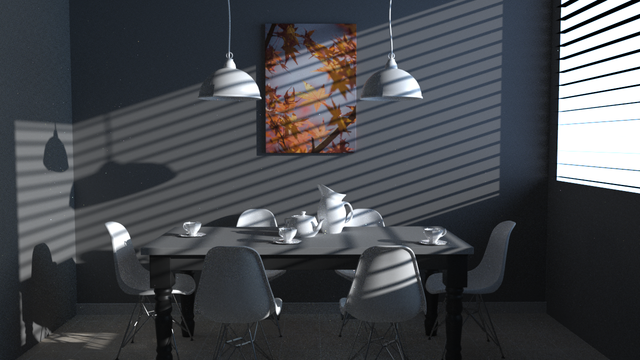
\includegraphics[width=0.32\linewidth]{images/5_results/dining_room/1_from_lux.png}
	\label{breakfast_Lux}	
}	
\subfloat[PBRT v3]{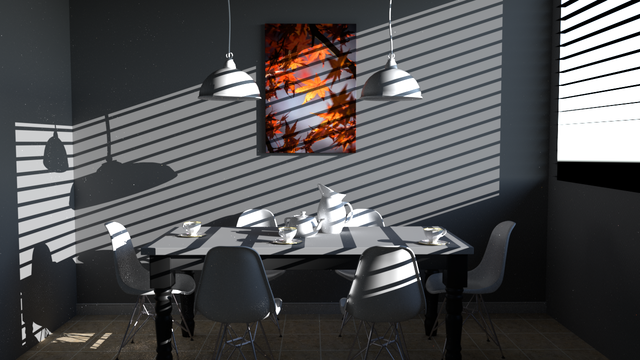
\includegraphics[width=0.32\linewidth]{images/5_results/dining_room/3_to_pbrt.png}
	\label{breakfast_PBRT}		
}	
\subfloat[Mitsuba]{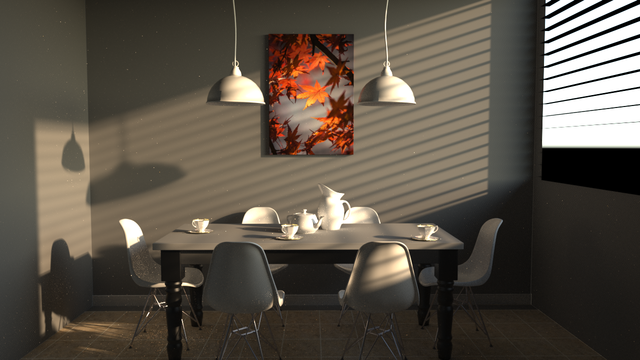
\includegraphics[width=0.32\linewidth]{images/5_results/dining_room/2_to_mitsuba.png}
		\label{breakfast_Mitsuba}	
}	
\caption{\textit{The Breakfast Room} scene. Input scene description for LuxRender (a).
	Renderings produced by PBRT v3 (b) and Mitsuba (c),
	from scene descriptions converted by our system. Mitsuba's sun directive produces a warm-colored lighting.}
\label{fig:dining-room}
\end{figure*}

\begin{figure}
	\centering
	\subfloat[Mitsuba]{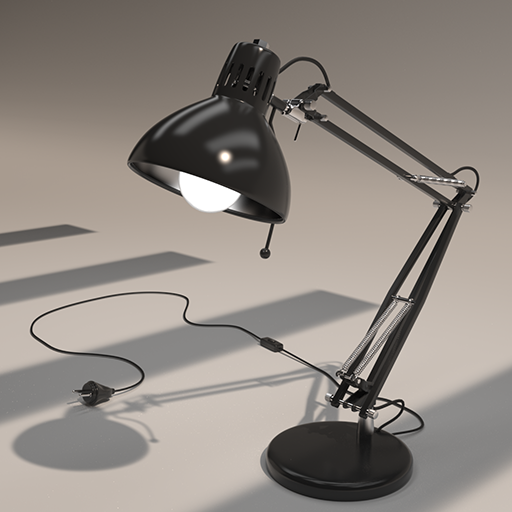
\includegraphics[width=0.32\linewidth]{images/5_results/lamp/1_from_mitsuba_s.png}
		\label{lamp_Mitsuba}	
	}	
	\subfloat[PBRT v3]{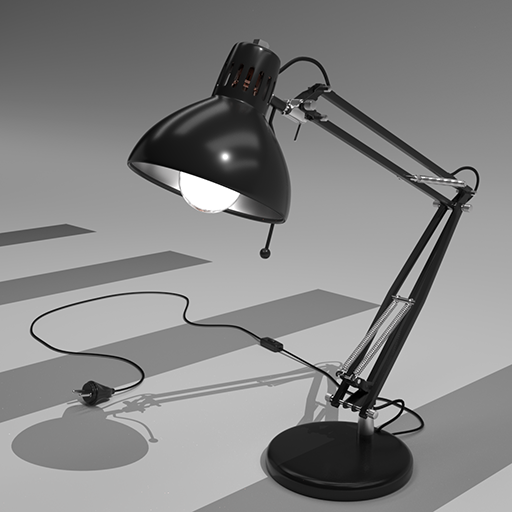
\includegraphics[width=0.32\linewidth]{images/5_results/lamp/2_to_pbrt_s.png}
		\label{lamp_PBRT}		
	}	
	\subfloat[LuxRender]{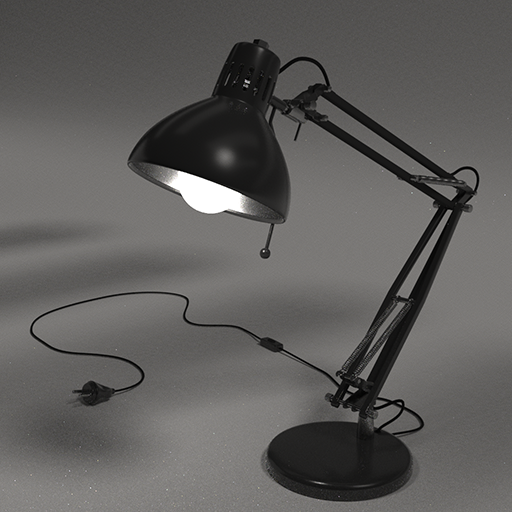
\includegraphics[width=0.32\linewidth]{images/5_results/lamp/3_to_lux_s.png}
		\label{lamp_Lux}	
	}	
	\caption{\textit{Little Lamp} scene. Input scene description for Mitsuba (a).
		Renderings produced by PBRT v3 (b) and LuxRender (c),
		from scene descriptions converted by our system. }
	\label{fig:lamp}
\end{figure}

\begin{figure}
	\centering
	\subfloat[PBRT v3]{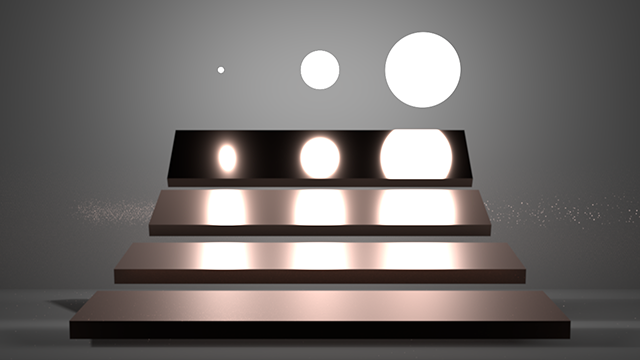
\includegraphics[width=0.32\linewidth]{images/5_results/veach-mis/1_from_pbrt_s.png}
		\label{MIS_PBRT}		
	}	
	\subfloat[Mitsuba]{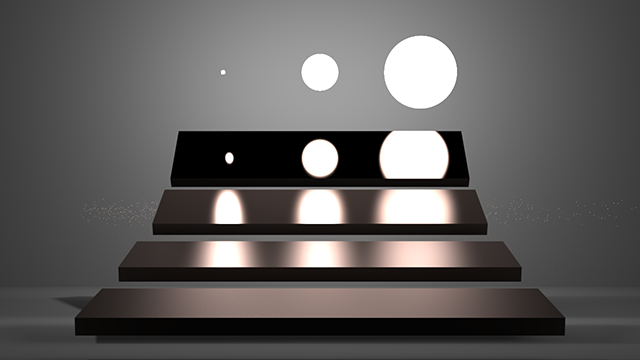
\includegraphics[width=0.32\linewidth]{images/5_results/veach-mis/2_to_mitsuba_s.png}
		\label{MIS_Mitsuba}		
	}	
	\subfloat[LuxRender]{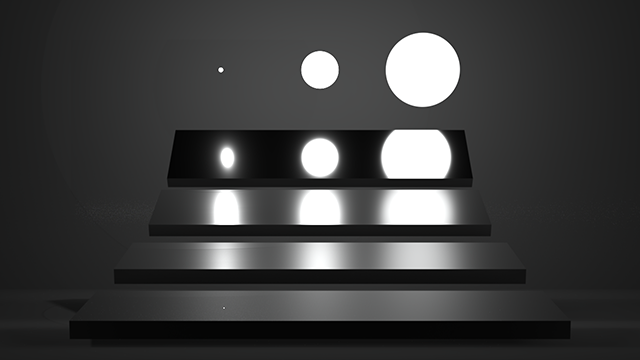
\includegraphics[width=0.32\linewidth]{images/5_results/veach-mis/3_to_lux_s.png}
		\label{MIS_Lux}		
	}	
	\caption{\textit{Veach, MIS}. 
		Renderings by PBRT v3 (a), Mitsuba (b), and LuxRender (c).
		Converting metal colors to LuxRender is a challenging task, not currently supported by our system. } 
	\label{fig:MIS}
\end{figure}

%\begin{figure}
%\centering
%\subfloat[PBRT v3]{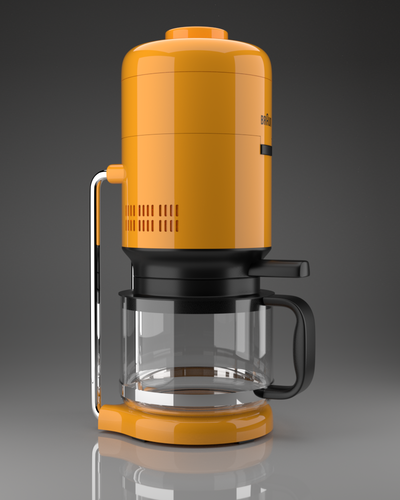
\includegraphics[width=0.32\linewidth]{figs/4_results/glass_of_water/1_from_pbrt.png}
%	\label{glass_PBRT}		
%}	
%\subfloat[LuxRender]{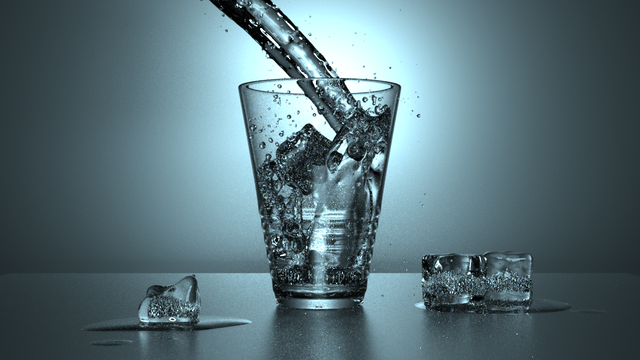
\includegraphics[width=0.32\linewidth]{figs/4_results/glass_of_water/2_to_lux.png}
%	\label{glass_Lux}		
%}	
%\subfloat[Mitsuba]{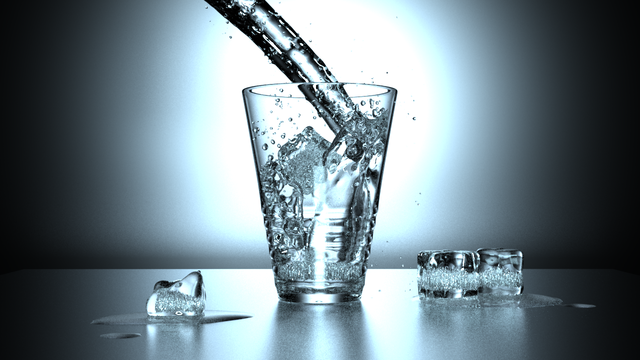
\includegraphics[width=0.32\linewidth]{figs/4_results/glass_of_water/3_to_mitsuba.png}
%	\label{glass_Mitsuba}		
%}	
%\caption{\textit{Glass of Water}. Input scene description for PBRT v3 (a).
%	Renderings produced by LuxRender (b) and Mitsuba (c),
%	from scene descriptions converted by our system. } 
%\label{fig:glass-of-water}
%\end{figure}





